\subsection{Forced-response stability and clearance boundaries}
\label{sec:stability-boundary}
To distinguish resonance amplification from a dynamical loss of stability,
we additionally scan the same nominal beam under a prescribed transverse
field. This experiment concerns attracting responses of a driven, damped
system; it does not measure destruction of the conservative KAM torus.
The physical parameters, frozen static-field modes and mass-drag coefficient
$\alpha=0.5555852368\,\mathrm{s}^{-1}$ are unchanged. No field-gradient
input, learned-model substitution, governor or contact force is used.
In physical time, the retained modal equations are
\begin{equation}
\begin{aligned}
 \dot X_j&=\omega_jY_j,\\
 \dot Y_j&=-\omega_jX_j-\alpha Y_j\\
 &\quad+\omega_0d_j[\vartheta-\sin\vartheta+u(t)\cos\vartheta],
\end{aligned}
\label{eq:boundary-modal-plant}
\end{equation}
where $\vartheta=d^{\mathsf T}X$, $u=B_y/B_0$, $B_0=30$ mT and
$\omega_0=11.417287283\,\mathrm{rad\,s^{-1}}$.

\paragraph{Fixed protocol and stability diagnostics.}
Independent runs use
$B_y=A[1-\exp(-(t/(0.25\,\mathrm{s}))^2)]\sin(r\omega_0t)$.
The amplitude set is $A\in\{1,2,4,6,10,15,20\}$ mT.
The frequency set contains the $0.02$ grid over $[0.70,1.30]$ and
the $0.005$ grid over $[0.94,1.06]$, giving $49$ distinct ratios.
For each pair, the initial low state is either zero or
$\pm(0.18,0.04,0,0)$, giving $1029$ independent integrations.
Increasing- and decreasing-frequency continuations add $686$ runs.
Each continuation changes frequency at the zero-field phase and inherits
the previous endpoint; the ramp is applied only at its first frequency.
Each run discards $128$ forcing periods and measures the next $64$,
for a total duration of $81.28$--$150.95$ s. Fixed-step DOP853 uses
$256$ steps per forcing period in the two-mode grid.

We integrate the analytic variational equation simultaneously, renormalize
one tangent vector every period, and average its logarithmic growth over
the last $64$ periods. These conditional finite-time Lyapunov exponents
hold the prescribed forcing phase fixed. We also integrate the complete
$4\times4$ fundamental matrix over a further period with $512$ steps,
and calculate the Floquet multipliers of every converged two-mode orbit.
The nontrivial Jacobian block is
\begin{equation}
 D_X\dot Y=-\operatorname{diag}(\omega_j)
 +\omega_0[1-\cos\vartheta-u\sin\vartheta]dd^{\mathsf T}.
\label{eq:boundary-variational-block}
\end{equation}
The identity $\det\mathcal M=\exp(-2\alpha T)$ for its monodromy
matrix supplies an independent numerical check.

All $1715$ runs converge to forcing-periodic responses. The largest
single-period canonical residual is $6.65\times10^{-11}$; the maximum
endpoint differences among the three initial states and between the two
continuation directions are $2.31\times10^{-11}$ and
$4.01\times10^{-11}$, respectively. Conditional exponents in the
independent grid range from $-0.28046$ to $-0.27044\,\mathrm{s}^{-1}$.
Floquet spectral radii range from $0.803809$ to $0.889055$, with the
determinant identity accurate to $1.41\times10^{-14}$.
Fifteen cases at amplitudes $2$, $6$ and $20$ mT and frequency ratios
$0.8$, $0.95$, $1$, $1.05$ and $1.2$ retain periodic recurrence and
negative conditional exponents when both the integration time and
steps per period are doubled, and separately with four and eight modes.
The latter use $1024$ and $4096$ steps per period. Time refinement
changes the sampled two-mode steady peak by at most
$3.81\times10^{-7}$ mm. An independently written adaptive DOP853
implementation also agrees in canonical state to $3.13\times10^{-13}$
on three twelve-period checks.

These are numerical local-stability and basin checks at specified points,
not a proof over a continuous parameter set. Of the $1029$ independent
runs, $550$ keep their sampled whole-beam slope bound below $0.1$ rad
throughout startup and measurement. We use this value as a conservative
reporting screen for the small-slope model, not as a calibrated physical
validity threshold. Large-amplitude rows are retained in the data and
marked in Figure~\ref{fig:stability-boundaries}, but do not establish
physical device performance. No resolved multistability or chaos is
detected in this scan; neither a chaos threshold nor conservative-torus
breakup is inferred from it.

\paragraph{Full-model resonance and clearance contours.}
To resolve the operational boundary without high-mode truncation, we
separately calculate periodic responses using all $64$ frozen FE modes.
For $f=\vartheta-\sin\vartheta+u\cos\vartheta$ with Fourier coefficients
$f_k$ and $\Omega=r\omega_0$, the exact linear modal response is
\begin{equation}
 X_{j,k}=\frac{\omega_0\omega_jd_j f_k}
 {\omega_j^2-(k\Omega)^2+\mathrm i\alpha k\Omega}.
\label{eq:boundary-fourier-response}
\end{equation}
Iterating this response with the nonlinear force gives a numerical
periodic solution; its full nonlinear ODE residual is checked after
reconstructing $\vartheta=d^{\mathsf T}X$. Amplitude root-finding then
locates a $4$ mm peak-displacement crossing at $31$ of $35$ frequency
ratios; the remaining four ratios, $1.225$--$1.30$, have no such crossing
below $20$ mT on the calculated branch. Cubic-Hermite Bernstein bounds
cover every centreline point at each sampled phase. At every reported
crossing these spatial upper bounds equal the actual tip peak to
$8.9\times10^{-16}$ mm, so the contour also locates a tip reaching
$4$ mm in the numerical periodic solution.

\begin{table}[t]
\centering\small
\caption{Numerical $4$ mm crossing amplitudes in mT. Steady crossings
use all $64$ modes. Startup crossings use eight modes, zero initial
state, the stated $0.25$ s ramp, and $192$ forcing periods. They are
protocol-dependent response contours, not certified safe-field limits.}
\label{tab:stability-boundaries}
\begin{tabular}{rrr}
\toprule
$\Omega/\omega_0$ & Steady & Startup\\
\midrule
$0.8$ & $13.6362$ & $8.6513$\\
$0.9$ & $7.5005$ & $5.1882$\\
$1.0$ & $1.9168$ & $1.9169$\\
$1.1$ & $8.7909$ & $5.7662$\\
$1.2$ & $18.5936$ & $10.4455$\\
\bottomrule
\end{tabular}
\end{table}

The steady contour has a numerical minimum near
$r=0.999245$ ($\Omega=11.408664\,\mathrm{rad\,s^{-1}}$), at
$A=1.915911$ mT and a spatial slope bound of $0.06750$ rad.
Thus a $20$ mT actuator limit alone cannot ensure clearance near resonance.
At five representative crossings, increasing the Fourier phase grid
from $1024$ to $4096$ changes the peak by at most $0.00526\,\mu$m.
Comparisons with $2$, $4$, $8$, $16$ and $32$ modes are retained:
at these same inputs the two-mode peak differs from the full FE peak
by up to $67.73\,\mu$m, whereas the eight-mode discrepancy is below
$4.18\,\mu$m. Independent full-FE Radau integration from the computed
periodic states at $r=0.8,1,1.2$ agrees in tip position to
$1.11\times10^{-12}$ m over one period.

Startup overshoot imposes a different contour. The eight-mode startup
roots in Table~\ref{tab:stability-boundaries} use $512$ observation
phases per cycle; doubling time, integration resolution and observation
resolution at $r=0.8,1,1.2$ changes the peak by at most
$0.0678\,\mu$m. Full-FE integration from rest over the first $32$
periods, combined with the separately computed periodic response,
changes the checked peak by at most $2.44\,\mu$m. At $r=0.8$, the
approximately $8.6513$ mT request has a $2.5411$ mm full-FE steady
amplitude but reaches $4.0020$ mm during startup. This is a numerical
overshoot example with no wall-contact force. The continuous-time
input-work governor of Section~\ref{sec:unifiedsafety} remains the
proved clearance mechanism; the response contours explain why both
frequency and startup must enter a practical operating choice.

\begin{figure*}[t]
\centering
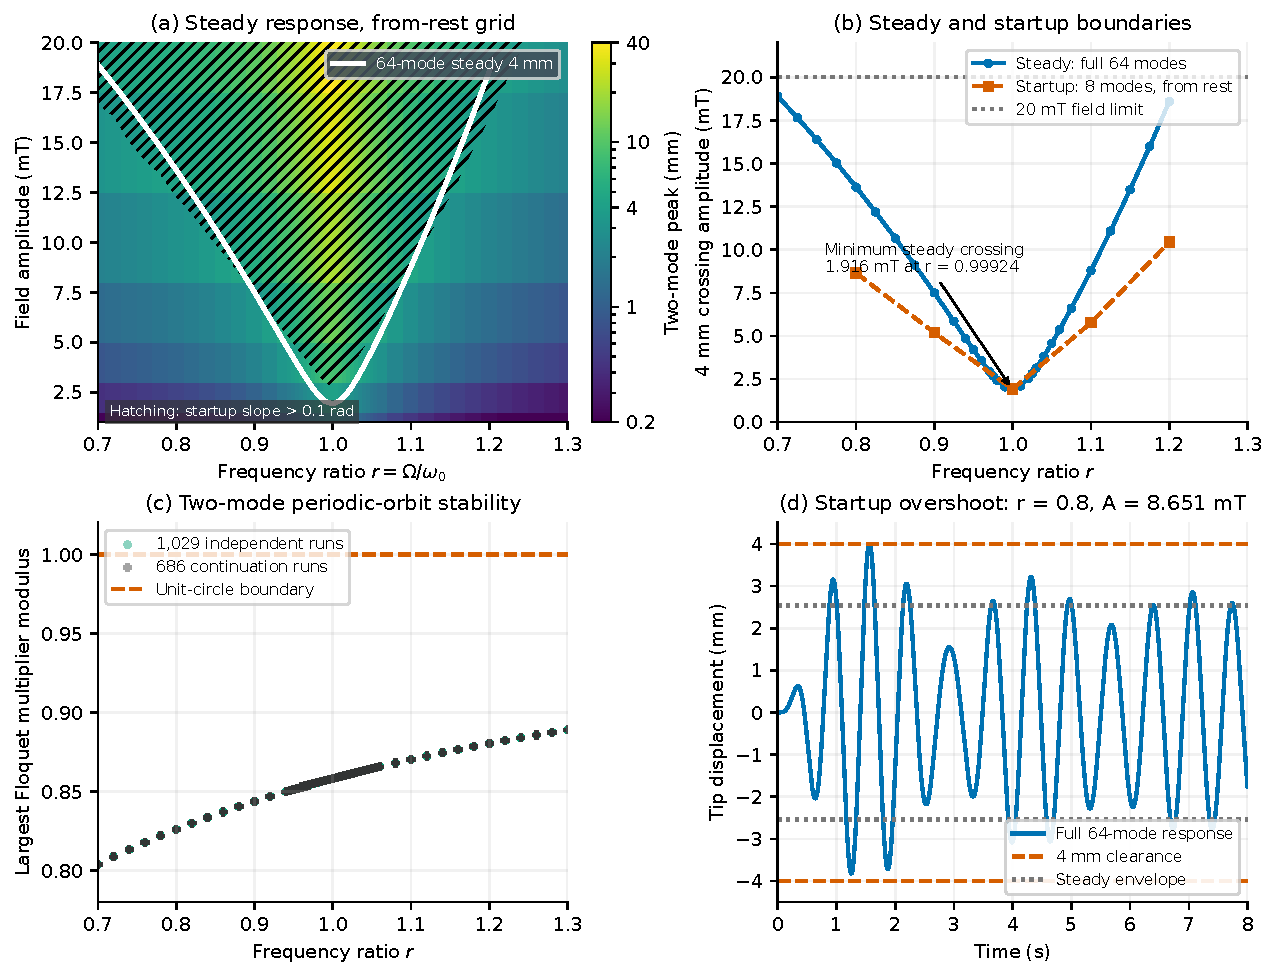
\includegraphics[width=\textwidth]{reproducibility/reviewer_revision_20261008/stability_scan/fig_stability_boundaries.pdf}
\caption{Driven-response and clearance study of the same magnetic beam.
(a) Two-mode steady peak on the from-rest grid; hatching marks sampled
startup slopes above the $0.1$ rad reporting screen. The white line is
the independently computed full-FE steady $4$ mm contour.
(b) Full-FE steady and eight-mode startup contours under the fixed ramp.
(c) Floquet multipliers of the two-mode periodic responses from all
independent and continuation runs. (d) Full-FE startup overshoot near
the eight-mode numerical crossing. Stability of an attracting forced
periodic response is distinct from conservative KAM-torus persistence.}
\label{fig:stability-boundaries}
\end{figure*}
